\chapter{Experiments}
\label{chapter:experiments}
    This chapter summarizes the setup of performed experiments and their results.

\section{Baselines}
\label{sub:exp-baseline}
    \noindent \textbf{DrQA:} We calculated the TF-IDF index using DrQA implementation for all unigrams and bigrams with $2^{24}$ buckets for hashing.
    
    \noindent \textbf{BM25:} We computed the index and then finetuned the \emph{k1} and \emph{b} hyper-parameters using grid search on defined grid \emph{k1} $\in$ [0.6, 1.2], \emph{b} $\in$ [0.5, 0.9] both with step 0.1. On a sample of 10,000 training claims, we selected the best performing parameter values: 
    \begin{table}[H] \label{table:bm25-hyperpar}
        \centering
        \begin{tabular}{lrr}
            dataset     &  \emph{k1}   & \emph{b}  \\
        \midrule
            FEVER CS    &  0.9  & 0.9  \\
            ČTK         &  0.6  & 0.5  \\
        \end{tabular}
    \end{table}

\section{ColBERT}
\label{sub:exp-colbert}
    We tried two setups here, 64-dimensional term representation with with document trimming to a maximum of 180 tokens and richer 128-dimensional term representation with document trimming to a maximum of 220 tokens on FEVER~CS. For the ČTK dataset we counted only the larger version, as it proved to be more powerful. The query is always truncated to a maximum of 32 tokens. 
    Training was done on triples (see section~\ref{sub:prop-colbert}) using two NVIDIA Tesla V100 GPU's with batch size 64, learning rate 3e-6, masked punctuation tokens, mixed precision and L2 similarity metric. %The latter representation provided slightly better results.

\section{Pretraining mBERT}
\label{sub:exp-pretrained}
    We used the cased multilingual mBERT from the HuggingFace library~\parencite{wolf-etal-2020-transformers} as the backbone model.

    \noindent \textbf{FEVER~CS:} The model was pretrained on ICT and BFS tasks on the Wikipedia articles for 20 epochs. The training was done on 4 GPUS's NVIDIA Tesla V100 with batch size 128, Adam optimizer with 1e-5 learning rate and no weight decay.
    In the finetuning phase was used the model from the pretraining phase that showed best performance on FEVER~CS development set. Then it was finetuned for next 20 epochs with the same setup except for learning rate, which was reduced to 5e-06 similarly to \parencite{chang2020twotower}. As a result, we saved the model with the highest performance on the development set.
    
    \noindent \textbf{ČTK:} We utilized the model already pretrained for 20 epochs on the Wikipedia (see above) and further pretrain it on the ČTK collection for 10 epochs with the same setup as stated above.
    In the finetuning phase, the model was finetuned using real claims and their annotated evidences for 20 epochs with 5e-06 learning rate and the rest of the setup remain unchanged.
    
    \begin{figure}[H]
        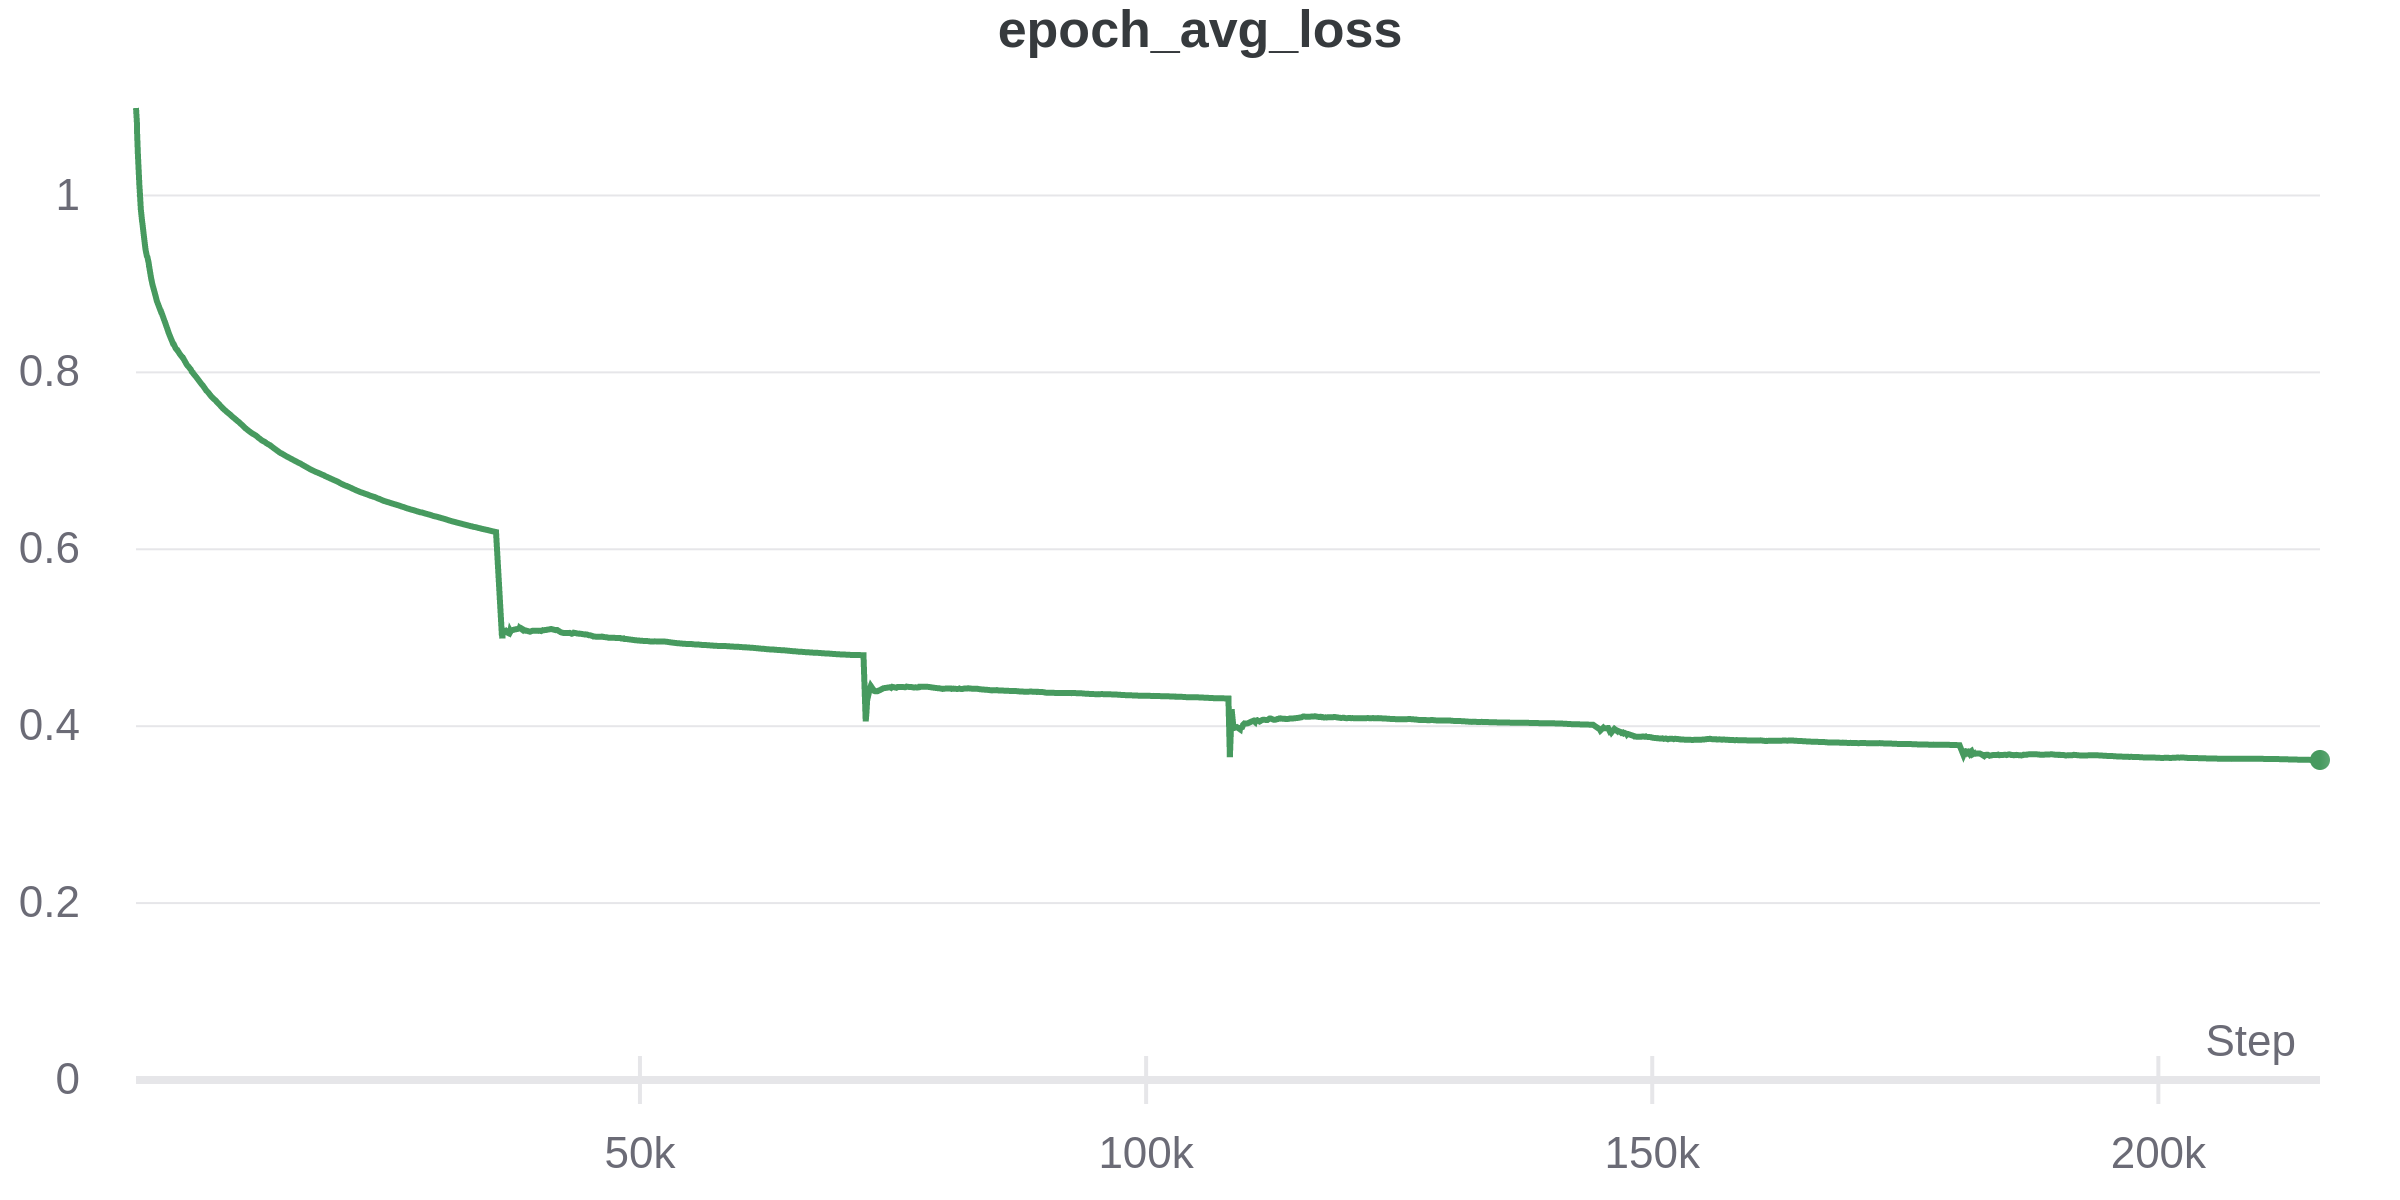
\includegraphics[width=0.8\linewidth]{mbert-ctk-pretraining.png}
        \centering
        \caption{Pretraining on ČTK learning curve}
        \label{fig:ctk-pretraining-lrcurve}
    \end{figure}
    
    \begin{figure}[H]
        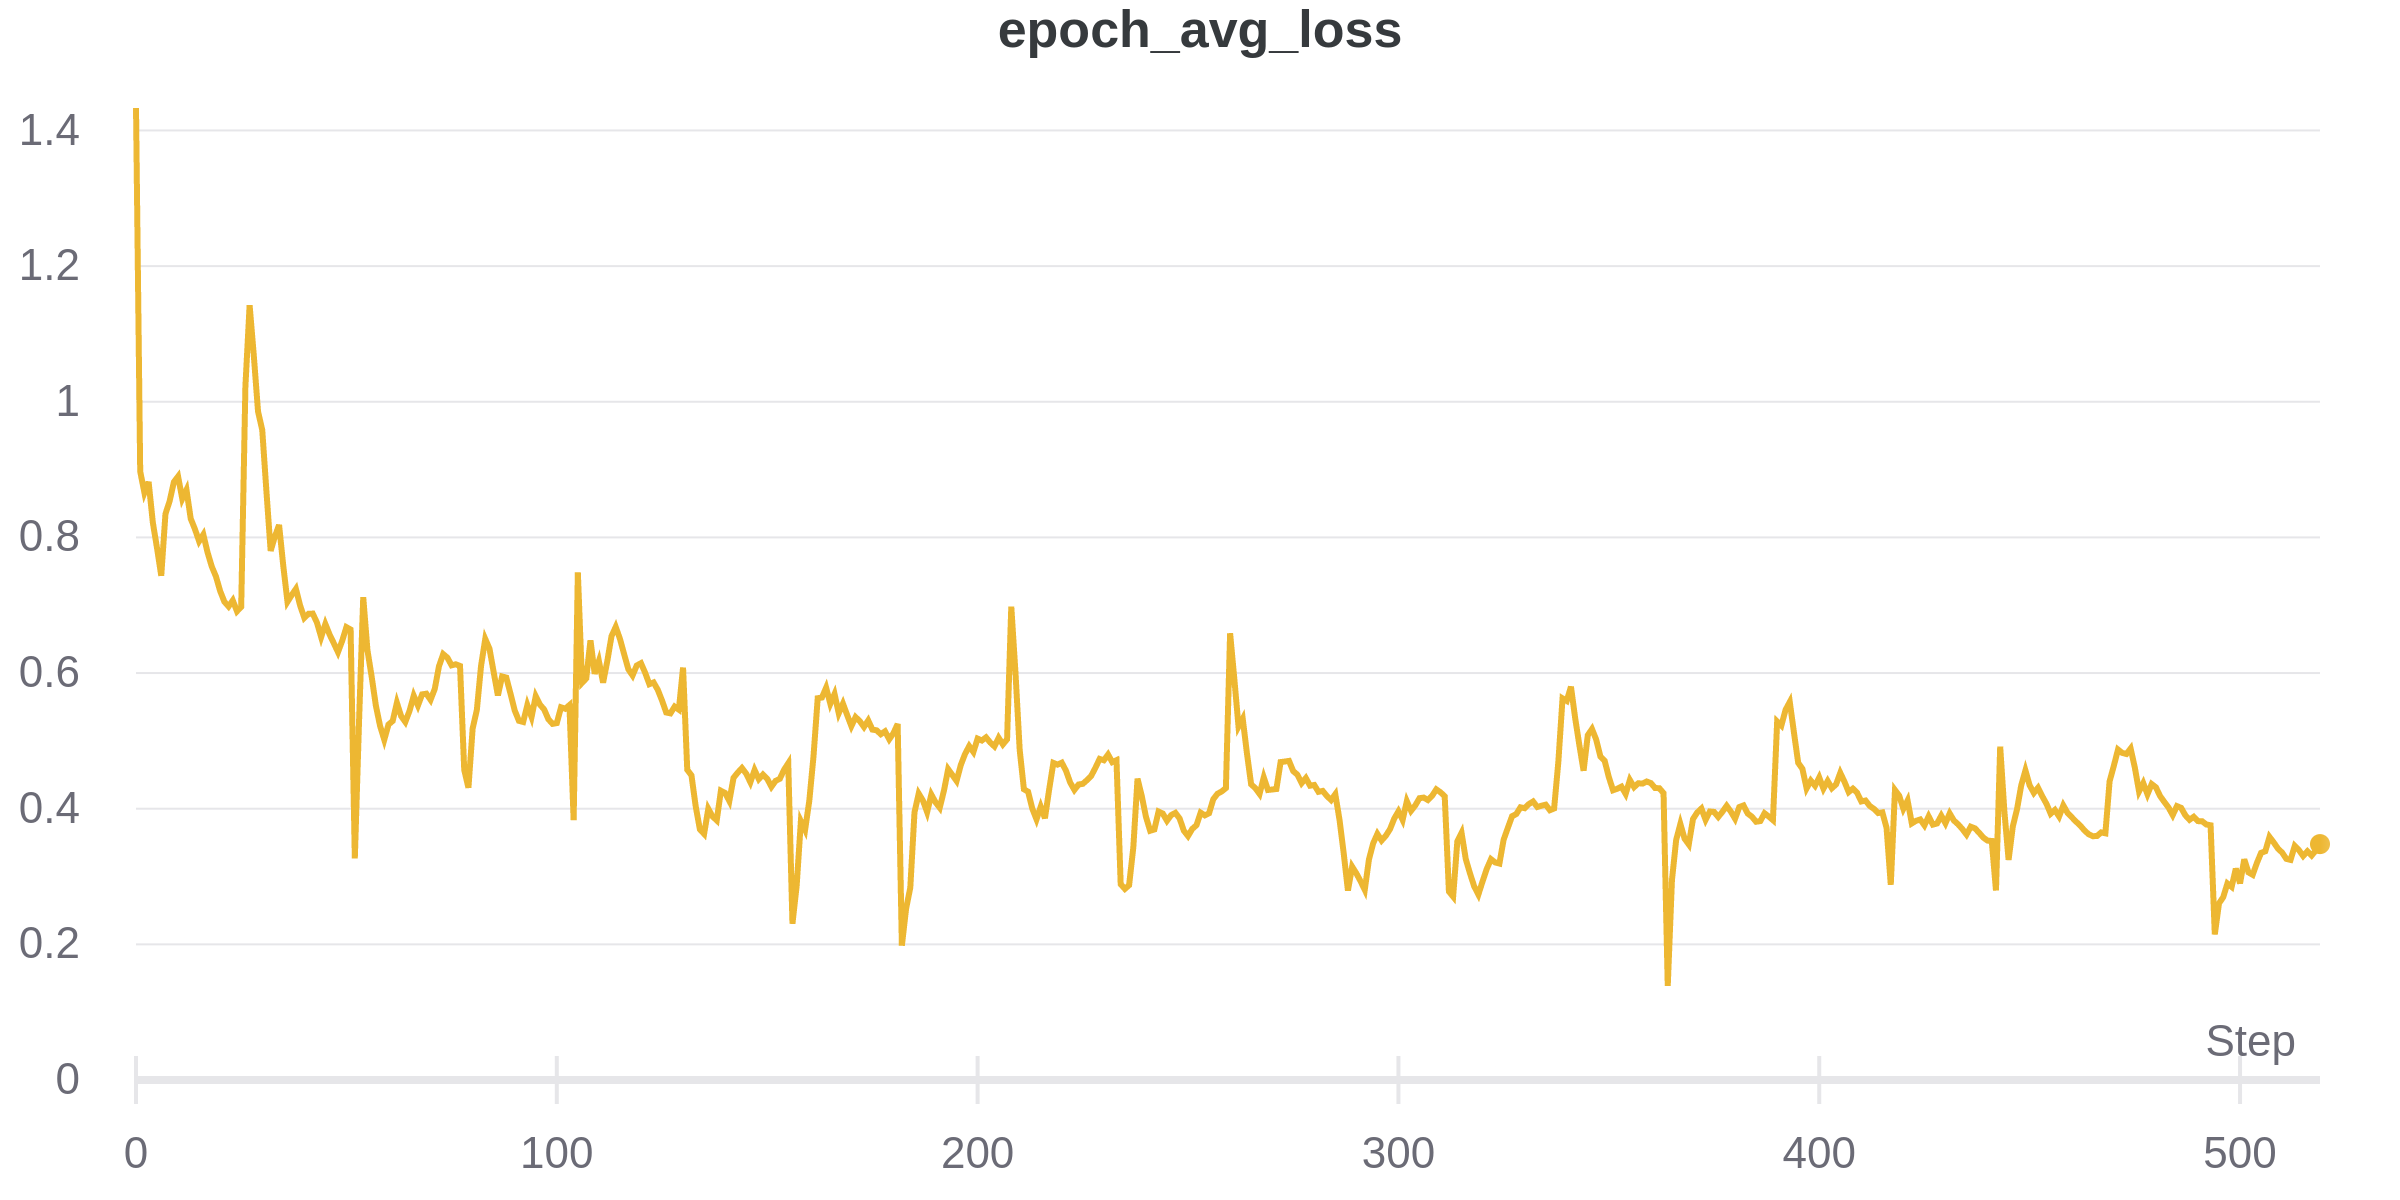
\includegraphics[width=0.8\linewidth]{mbert-ctk-finetuning.png}
        \centering
        \caption{Finetuning on ČTK learning curve}
        \label{fig:ctk-finetuning-lrcurve}
    \end{figure}
    
\section{Results}
\label{section:results}
% ----------------------------------------------------------------------------------------------------------
% FEVER
% ----------------------------------------------------------------------------------------------------------
\begin{table}[H] \label{table:fever-p}
    \centering
    \begin{tabular}{lrrrr}
    \toprule
                            model &    P@1 &    P@5 &   P@10 &  P@20 \\
    \midrule
                             DRQA &  42.42 &  13.66 &   7.56 &  4.08 \\
          Anserini BM25 finetuned &  41.24 &  13.12 &   7.37 &  4.02 \\
                    mBERT BFS+ICT &  \textbf{65.87} &  \textbf{19.13} &  \textbf{10.16} &  \textbf{5.28} \\
           ColBERT 128 (FEVER CS) &  56.33 &  15.45 &   8.20 &  4.29 \\
     ColBERT 128 (ČTK + FEVER CS) &  45.93 &  13.94 &   7.69 &  4.15 \\
      ColBERT 64 (ČTK + FEVER CS) &  44.21 &  13.20 &   7.28 &  3.93 \\
    \bottomrule
    \end{tabular}
    \caption{Precision at \emph{k} on FEVER~CS test set.}
\end{table}

\begin{table}[H] \label{table:fever-r}
    \centering
    \begin{tabular}{lrrrr}
    \toprule
                            model &    R@1 &    R@5 &   R@10 &   R@20 \\
    \midrule
                             DRQA &  39.14 &  62.39 &  68.89 &  73.99 \\
          Anserini BM25 finetuned &  38.12 &  60.41 &  67.43 &  73.18 \\
                    mBERT BFS+ICT &  \textbf{61.27} &  \textbf{87.43} &  \textbf{91.75} &  \textbf{94.48} \\
           ColBERT 128 (FEVER CS) &  52.39 &  71.48 &  75.38 &  78.40 \\
     ColBERT 128 (ČTK + FEVER CS) &  42.57 &  64.31 &  70.42 &  75.46 \\
      ColBERT 64 (ČTK + FEVER CS) &  41.24 &  60.98 &  66.88 &  72.01 \\
    \bottomrule
    \end{tabular}
    \caption{Recall at \emph{k} on FEVER~CS test set.}
\end{table}

\begin{table}[H] \label{table:fever-f1}
    \centering
    \begin{tabular}{lrrrr}
    \toprule
                            model &   F1@1 &   F1@5 &  F1@10 &  F1@20 \\
    \midrule
                             DRQA &  40.72 &  22.42 &  13.63 &   7.73 \\
          Anserini BM25 finetuned &  39.62 &  21.55 &  13.29 &   7.63 \\
                    mBERT BFS+ICT &  \textbf{63.49} &  \textbf{31.40} &  \textbf{18.29} &  \textbf{10.01} \\
           ColBERT 128 (FEVER CS) &  54.29 &  25.41 &  14.80 &   8.14 \\
     ColBERT 128 (ČTK + FEVER CS) &  44.19 &  22.91 &  13.86 &   7.86 \\
      ColBERT 64 (ČTK + FEVER CS) &  42.67 &  21.71 &  13.13 &   7.46 \\
    \bottomrule
    \end{tabular}
    \caption{F1 at \emph{k} on FEVER~CS test set.}
\end{table}

\begin{table}[H] \label{table:fever-mrr}
    \centering
    \begin{tabular}{lrrrr}
    \toprule
                            model &  MRR@1 &  MRR@5 &  MRR@10 &  MRR@20 \\
    \midrule
                             DRQA &  40.72 &  49.94 &   50.81 &   51.14 \\
          Anserini BM25 finetuned &  39.39 &  48.09 &   49.02 &   49.44 \\
                    mBERT BFS+ICT &  \textbf{57.57} &  \textbf{69.32} &   \textbf{70.05} &   \textbf{70.26} \\
           ColBERT 128 (FEVER CS) &  55.10 &  62.67 &   63.17 &   63.36 \\
     ColBERT 128 (ČTK + FEVER CS) &  44.48 &  53.18 &   53.92 &   54.28 \\
      ColBERT 64 (ČTK + FEVER CS) &  43.63 &  51.92 &   52.68 &   52.99 \\
    \bottomrule
    \end{tabular}
    \caption{Mean reciprocal rank at \emph{k} on FEVER~CS test set.}
\end{table}

% ----------------------------------------------------------------------------------------------------------
% CTK
% ----------------------------------------------------------------------------------------------------------
\begin{table}[H] \label{table:ctk-p}
    \centering
    \begin{tabular}{lrrrrr}
    \toprule
                              model &    P@1 &   P@5 &  P@10 &  P@20  \\
    \midrule
                               DRQA &  12.50 &  5.05 &  3.07 &  1.76  \\
            Anserini BM25 finetuned &  15.50 &  5.80 &  3.35 &  1.97 \\
           ColBERT 128 (FEVER CS + ČTK) &  \textbf{19.25}&  \textbf{7.00} &  \textbf{3.97} &  \textbf{2.29} \\
     mBERT BFS+ICT (FEVER CS + ČTK) &   0.75 &  0.95 &  0.80 &  0.60  \\
    \bottomrule
    \end{tabular}
    \caption{Precision at \emph{k} on ČTK test set.}
\end{table}

\begin{table}[H] \label{table:ctk-r}
    \centering
    \begin{tabular}{lrrrrr}
    \toprule
                              model &    R@1 &    R@5 &   R@10 &   R@20  \\
    \midrule
                               DRQA &  12.75 &  25.50 &  31.00 &  35.50  \\
            Anserini BM25 finetuned &  15.75 &  29.25 &  33.75 &  39.75  \\
           ColBERT 128 (FEVER CS + ČTK) &  \textbf{19.50} &  \textbf{35.25} &  \textbf{40.00} &  \textbf{46.00} \\
     mBERT BFS+ICT (FEVER CS + ČTK) &   1.00 &   5.00 &   8.25 &  12.25 \\
    \bottomrule
    \end{tabular}
    \caption{Recall at \emph{k} on ČTK test set.}
\end{table}

\begin{table}[H] \label{table:ctk-f1}
    \centering
    \begin{tabular}{lrrrrr}
    \toprule
                              model &   F1@1 &   F1@5 &  F1@10 &  F1@20  \\
    \midrule
                               DRQA &  12.62 &   8.43 &   5.60 &   3.36 \\
            Anserini BM25 finetuned &  15.62 &   9.68 &   6.10 &   3.76 \\
           ColBERT 128 (FEVER CS + ČTK) &  \textbf{19.37} &  \textbf{11.68} &   \textbf{7.23} &   \textbf{4.36} \\
     mBERT BFS+ICT (FEVER CS + ČTK) &   0.86 &   1.60 &   1.46 &   1.14 \\
    \bottomrule
    \end{tabular}
    \caption{F1 at \emph{k} on ČTK test set.}
\end{table}

\begin{table}[H] \label{table:ctk-mrr}
    \centering
    \begin{tabular}{lrrrrr}
    \toprule
                              model &  MRR@1 &   MRR@5 &  MRR@10 &  MRR@20  \\
    \midrule
                               DRQA &  13.05 &  17.72 &   18.31 &   18.60  \\
            Anserini BM25 finetuned &  15.79 &   20.40 &   20.95 &   21.36  \\
           ColBERT 128 (FEVER CS + ČTK) &  \textbf{18.32} &   \textbf{24.21} &   \textbf{24.85} &   \textbf{25.26}  \\
     mBERT BFS+ICT (FEVER CS + ČTK) &   1.47 &    2.78 &    3.12 &    3.45  \\
    \bottomrule
    \end{tabular}
    \caption{Mean reciprocal rank at \emph{k} on ČTK test set.}
\end{table}